\documentclass[11pt]{article}
\setlength{\oddsidemargin}{0in}
\setlength{\evensidemargin}{0in}
\setlength{\textwidth}{6.5in}

\usepackage{fancyhdr}
\pagestyle{fancy}
\usepackage{amsmath,amsfonts,amssymb}
\usepackage{epsfig}
\usepackage{subfigure}
\usepackage{placeins}
\usepackage{amsmath}
\usepackage[usenames,dvipsnames,svgnames,table]{xcolor}
\usepackage{amssymb}
\usepackage{setspace}
\usepackage{graphicx} % Include figure files
\usepackage{times}
\usepackage{amsthm}
\usepackage{hyperref}
\usepackage{enumitem}
\hypersetup{bookmarks=true, unicode=false, pdftoolbar=true, pdfmenubar=true, pdffitwindow=false, pdfstartview={FitH}, pdfcreator={Daniel Larremore}, pdfproducer={Daniel Larremore}, pdfkeywords={} {} {}, pdfnewwindow=true, colorlinks=true, linkcolor=blue, citecolor=Green, filecolor=magenta, urlcolor=cyan,}
\usepackage[parfill]{parskip}
\usepackage{tcolorbox}
\tcbuselibrary{breakable}
\usepackage{float}

% This little bit tells LaTeX where to look for figures.
% As written, it says to look first in Notes/figs_python, and then look in the current directory ./  
\graphicspath{{../Notes/figs_python/}{./}}

\begin{document}

\lhead{{\bf Mathematical \& Computational Modeling of Infectious Diseases \\ 
Homework 1}}
\rhead{{\bf D.B.\ Larremore\\2024}}
\renewcommand{\headrulewidth}{0.4pt}

{\bf Instructions:} 
\begin{itemize}[itemsep=-7pt]
	\item Please turn in a single PDF file.
	\item Please share a link to your code, but do not attach the actual code. 
	\item {\color{blue} By the way, if you don't have a github, why not make one? It's easy to do, and a great place to stash your code and link to it. Pop by office hours or phone a friend if you need help. It's never too early (or late) to learn!} 
	\item Handwritten math (scanned and included in a PDF) is fine, but please avoid 10MB+ file sizes! Reduce your image quality as needed. 
	\item Don't forget to list anyone you collaborated with. 
\end{itemize}
\vspace{0.1in}\hrule

\begin{enumerate}

\item The goal of this problem is to get you over any barriers with (i) getting Python set up, (ii), getting the SIR model implemented in a Forward Euler solver, and (iii) getting matplotlib set up.
	
	Write a function in Python that uses the Forward Euler method to simulate the SIR model. Check your work by first reproducing the three plots from Figure 1 of the Week 2 lecture notes. The parameters are: $N=1000$, $I_0=1$, $S_0=999$, with 
	\begin{itemize}
		\item $\beta=1$, $\gamma=0.5$
		\item $\beta = 1.5$, $\gamma=0.5$
		\item $\beta = 2$, $\gamma=0.5$
	\end{itemize}
	Show that your code works by simply reproducing the plots exactly, but with your first name included in the legend labels, e.g. ``S Dan'', ``I Dan'' or something. Link to your code and turn in just the 3 plots. 
	
	\begin{tcolorbox}[breakable]
		\textbf{Solution:} Here, I have reproduced the plots using forward Euler
	\end{tcolorbox}

	\begin{figure}[H]
		\centering
		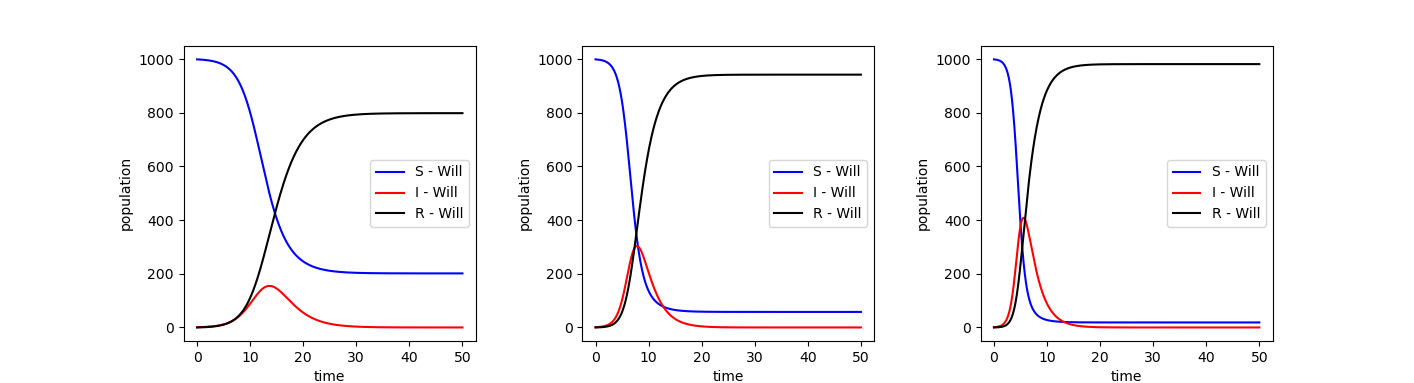
\includegraphics[scale=0.5]{p1.png}
		\caption{Simulations of SIR models. $\gamma=0.5$, $N=1000$, $\beta$ from left to right is $1, 1.5,2$ resp.}
	\end{figure}
	
\clearpage
\item The goal of this problem is to show an important fact about transition rates in compartmental models. It is also a good chance to become refreshed on simple ODE solving and separation of variables. Finally, it makes good on a promise made in Week 2's lecture notes to ask this homework question!
	
	Imagine that we are interested in SIR dynamics, but everyone starts out either infected or recovered, and no one starts out susceptible.
	\begin{enumerate}[label=\alph*.]
		\item Use this information to simplify the typical equation for $\dot{I}$.
		\begin{tcolorbox}[breakable]
			\textbf{Solution:}
			Beginning with the standard homogeneous mixing SIR model we have that
			\begin{align*}
				\dot{S} &= -\beta S I\frac{1}{N}\\
				\dot{I} &=\beta S I\frac{1}{N} - \gamma I\\
				\dot{R} &= \gamma I\\
				&S(0), \, I(0), \, R(0)= S_0, \,I_0, \,R_0.
			\end{align*}
			Per the problem statement, we have that at $t=0$, we have the number of susceptible individuals is $S_0=0$ and the remaining are either infected or recovered/removed, that is $I_0+R_0=N$. Since there is no way to enter the susceptible category, $S(t)=0, \, \forall t\geq0$. This reduces the equations to 
			\begin{align*}
				S &= 0\\
				\dot{I} &= - \gamma I\\
				\dot{R} &= \gamma I\\
				&S(0), \, I(0), \, R(0)= 0, \,I_0, \,R_0.
			\end{align*}
			Since $I(t)+R(t)=N$ is a constant, $R$ is fully characterized by $I$, so we now only require one equation, the infected equation, to characterize the system, that is
			\begin{align*}
				\dot{I}(t)=-\gamma I, \, I(0)=I_0 \in [0, N]
			\end{align*}
		\end{tcolorbox}
		\item Solve your simplified differential equation with the initial condition $I(0) = I_0$.
		\begin{tcolorbox}[breakable]
			\textbf{Solution:}
			Solving our simplified equation, 
			\begin{align*}
			\dot{I}(t)=-\gamma I, \, I(0)=I_0 \in [0, N],
			\end{align*}
			we may use one of many methods, the simplest is separation of variables. To be explicit, we have
			\begin{align*}
				\dot{I}(t)&=-\gamma I(t)\\
				e^{\gamma t}\dot{I}(t) &+\gamma e^{\gamma t} I(t)=0\\
				\frac{\rm d}{\rm d t}e^{\gamma t}I(t) = 0\\
				e^{\gamma t}I(t) &= K\\
				I(t)&=K e^{-\gamma t}\\
				I(0)&=I_0=K\\
				I(t)=I_0 e^{-\gamma t}.
			\end{align*}
			This indicates that, since $\gamma \geq 0$, the infected load either remains constant or decays exponentially with time constant $1/\gamma$.
		\end{tcolorbox}
		\item Manipulate your solution to derive the fraction of the initially infected people who are still infected at time $t$.
		\begin{tcolorbox}[breakable]
			\textbf{Solution:}
			Taking our exponential decay solution, we solve for the fraction of infected people by dividing by $N$.
			\begin{align*}
				I(t)&=I_0e^{-\gamma t}\\
				i(t)&=\frac{I(t)}{N} = \frac{I_0}{N}e^{-\gamma t}\\
				i(t)&=i_0 e^{-\gamma t}.
			\end{align*}
		\end{tcolorbox}
		\item Discuss this equation. What does it do over time? How is it related to the fraction of infected people who have {\it left} the infected class?
		\begin{tcolorbox}[breakable]
			\textbf{Solution:}
			As long as $\gamma >0$, this indicates that the fraction of infected persons decays exponentially. Recall that the sum of the infected and recovered frations is $1$, that is 
			$i+r=1$, so then 
			\begin{equation*}
				r(t)=1-i(t) = 1-i_0e^{-\gamma t} =1-(1-r_0)e^{-\gamma t},
			\end{equation*}
			which indicates that the fraction of recovered persons decays to $1$, that is, everyone eventually entered the recovered category given sufficiently long time.
		\end{tcolorbox}
		\item This formula produces values between $0$ and $1$, and it tells us the probability that a randomly chosen infected person is still infected at time $t$. How does this relate to the cumulative distribution function (CDF) that describes the probability that someone is infected for less than or equal to $t$ units of time? Take a derivative of the CDF to get a PDF for the duration of infection lengths is. Then, find out what this famous probability distribution is called, and write down its expected value.
		\begin{tcolorbox}[breakable]
			\textbf{Solution:}
			We may solve this by assuming that in a given time period, $\rm d t$, the proportion of infected that recover is $\gamma \rm d t$. Then, if we want to figure out if an individual originally infected recovers by some time $T$, we break $T$ into $M$ sections of length $\rm d t$ such that $T=M \rm d t$. After time interval $\rm d t$ the probability the infected person does not recover is $\sim1-\gamma \rm d t$. After $K$ time intervals, the probability the person has not recovered is $\sim (1- \gamma \rm d t)^K$, and finally, the probability that the person has not recovered by time $T$ is $(1-\gamma \rm d t)^M=(1-\gamma \frac{1}{M})^M)$. Taking the limit of breaking the intervals into arbitrarily many sub intervals gives
			\begin{equation*}
				P(\text{Has not recovered by time }T) = \lim_{M\rightarrow \infty}(1-\frac{\gamma}{M})^M = e^{-\gamma T}.
			\end{equation*}
			Then the cumulative density function is 
			\begin{equation*}
				CDF(t) = 1-e^{-\gamma t}.
			\end{equation*}
			Taking derivatives to find the probability density function gives
			\begin{equation*}
				PMF(t) = \frac{\rm d}{\rm d t} = 1-e^{-\gamma t} = \gamma e^{-\gamma t},
			\end{equation*}
			which is the exponential distribution. This yields the expected time to recovery as
			\begin{equation*}
				\langle t \rangle = \int_0^\infty \gamma t e^{-\gamma t} = \frac{1}{\gamma},
			\end{equation*}
			as is expected.
		\end{tcolorbox}
		\item Use your results to explain how the recovery rate $\gamma$ is related to the typical amount of time a person remains infectious.
		\begin{tcolorbox}[breakable]
			\textbf{Solution:}
			The expected value can be interpreted as, on average, how long one is expected to remain in the "Infected" category, and hence how long the model expects an individual to be infectious.
		\end{tcolorbox}
	\end{enumerate}

\clearpage
\item The goal of this problem is to (i) figure out how to solve the final epidemic size equation, and (ii) test the equation's predictions.

	\begin{enumerate}[label=\alph*.]
		\item First, explain how an epidemic's total size, also called its cumulative incidence, is related to $s_\infty$ and $r_\infty$. 
		\begin{tcolorbox}[breakable]
			\textbf{Solution:}
			Here, we recall that $S+I+R=N$ where $N$ is the total population in question, and assuming that $\dot{N}=0$. Then, dividing, we have that 
			\begin{equation*}
				S+I+R=N \implies \frac{S+I+R}{N}=1=s+i+r.
			\end{equation*}
			The cumulative number of infections over the lifetime of the disease is then $I_\infty/N = i = 1-s_\infty-r_\infty$.
		\end{tcolorbox}
		\item Recall that $r_\infty = 1-e^{-R_0 r_\infty}$. Though we can't solve this equation, we can use a
		 valuable graphical technique: if we set $f(r_\infty) = r_\infty$ and $g(r_\infty) = 1-e^{-R_0 r_\infty}$, we can plot both $f(r_\infty)$ vs $r_\infty$ and $g(r_\infty)$ vs $r_\infty$, and see where $f=g$. Create four plots for $R_0 \in \{0.9, 1.0, 1.1, 1.2\}$ with $f$ in black and $g$ in red. Use the {\bf fsolve} function to find the intersection point, and use matplotlib's {\bf scatter} function to plot a blue circle at the intersection.\footnote{Hint, use \href{https://docs.scipy.org/doc/scipy/reference/generated/scipy.optimize.fsolve.html}{the fsolve docs}, and note that, because fsolve wants to find roots (points where a function is zero), you can create an auxiliary function $h(r_\infty) = f(r_\infty)-g(r_\infty)$ which will be equal to zero at the point where $f$ and $g$ intersect!}
		\begin{tcolorbox}[breakable]
			\textbf{Solution:}
			Here, we use Python to produce the images as required below.
		\end{tcolorbox}
		\begin{figure}[H]
			\centering
			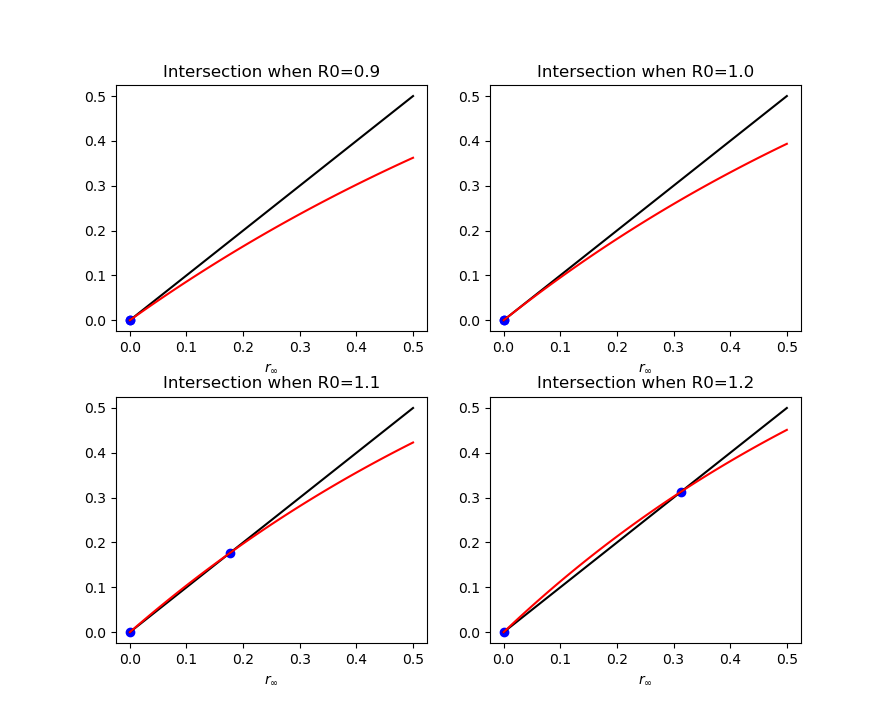
\includegraphics[scale=0.75]{3b.png}
			\caption{Plots of numerical solutions as the basic reproduction number increases. Multiple solutions only occur once $R_0>1$.}
		\end{figure}
		\item Comment on what you see in the plots in the context of what we have learned about $R_0$. What do you see in your figures? What happens when $R_0 < 1$ ?
		\begin{tcolorbox}[breakable]
			\textbf{Solution:}
			The interpretation of $R_0$ as "the number of secondary infections per primary infection" is instructive here. Supposing that $R_0<1$, and starting with a single primary infection, you will not be able to infect any other individuals (since you can not infect part of a person), so there will only ever be the primary individual that goes into the recovery category, which is a negligibly small fraction of the population, of $r_\infty\sim 0$. Similarly, supposing that $R_0>1$, then you will always infect at least enough people to replace yourself, so the number of infected individuals will always increase until the susceptible population is small enough for the infection rate to die off and the recovered population will saturate at some non-zero fraction. 
		\end{tcolorbox}
		\item Finally, test the predictions made by this final-size equation by using your SIR code and $\beta=1$, $\gamma=0.5$ by creating a new version of that epidemic with a green dotted line at the height of $r_\infty$. Does this final size prediction work?\footnote{Take care, as the units of our SIR plots and the units of our final size prediction are not the same! You may have to do a conversion...}
		\begin{tcolorbox}[breakable]
			\textbf{Solution:}
			Given the parameter set $(\beta, \gamma)=(1, 0.5)$ gives that $R_0=\frac{\beta}{\gamma}=2$. This parameter set was used for problem 1. From the simulation, we have that $(S_\infty, I_\infty, R_\infty)\sim(201.5,0,798.5)$, so ignoring the fact that there are fractional people and converting into population densities gives $(s_\infty, i_\infty, r_\infty)\sim(0.2015,0,0.7985)$. Using our rootsolver, we get a value of $\overline{r_\infty}\sim  0.79681213$, which is very close to the simulated value, giving less than a percent error between them, which is likely due to numerical error and finite size timesteps from the Euler method.
		\end{tcolorbox}
	\end{enumerate}
	

\clearpage
\item (Grad / EC): In class, we showed that the SIR model's disease-free equilibrium is stable when $s<\tfrac{1}{R_0}$ and unstable otherwise. Using $N=10^6$, and $\varepsilon = \frac{1}{N}$ as your perturbation, produce a single figure {\it using your simulation code and its output} that illustrates this point. Write a caption that explains the principle of stability, and explain how your figure illustrates it.\footnote{There are many possible ways to make such a figure, and write its caption! One could use all of the outputs of the simulation, for instance, but one could also use just those that illustrate the intended point.}
\begin{tcolorbox}[breakable]
	\textbf{Solution:}
	Here we will take the case that $(\beta, \gamma)=(1, 0.5)$ which makes $R_0=2$. This means that we should expect when the remaining susceptible fraction of population is less than $1/R_0$, that is $s<1/2$, then the fraction of infected population should decay back to $0$. To demonstrate this phenomena, we will take initial conditions of $(s_0, i_0, r_0)=(0.4, \epsilon, 0.6-\epsilon)$, where I have removed a fraction$\epsilon$ from the recovered fraction to maintain the requirement that $s+i+r=1$ when the system is perturbed from its prior implied equillibrium of $(0.4, 0, 0.6)$. We expect this figure to have the infected fraction decay to $0$. In Fig. \ref{im:log}, we have plotted the diagram on a log-scale to make the decay of $I(t)$ to 0 more evident. Note that by perturbing the number of infected by $1$ person, it immediately begins decaying away, leaving the susceptible unchanged and the number of recovered will eventually only increase by $1$. This corroborates the expected behavior.
\end{tcolorbox}

\begin{figure}[H]
	\centering
	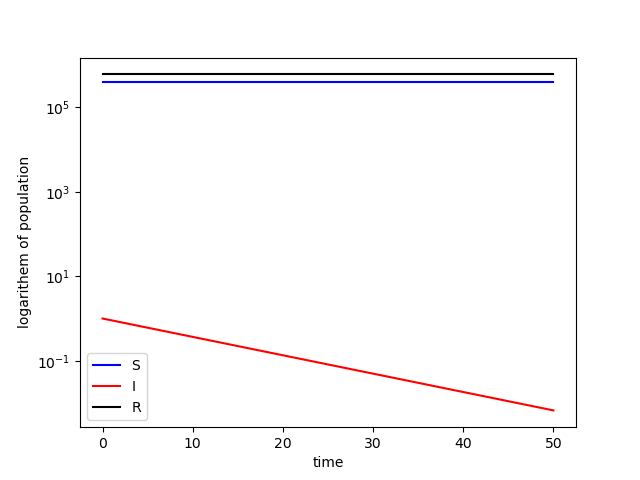
\includegraphics[scale=0.7]{p4.png}
	\label{im:log}
\end{figure}

\end{enumerate}



\end{document}